\documentclass[11pt]{article}
\usepackage[T1]{fontenc}
\usepackage[margin=1in]{geometry}
\usepackage{amsmath,amssymb,amsthm}
\usepackage{graphicx}
\usepackage[colorlinks=true,linkcolor=blue,citecolor=blue,urlcolor=blue]{hyperref}
\theoremstyle{remark}
\newtheorem{remark}{Remark}[section]
\newcommand{\Tr}{\operatorname{Tr}}
\newcommand{\deff}{d_{\rm eff}}
\newcommand{\dmax}{d^{\max}_{\rm eff}}

\title{Finite-Size Scaling of Petz Recovery Length in the TFIM\\
{\large Threshold-dependent operational exponents from exact
diagonalization}\\
{\normalsize Version 2}}
\author{Lluis Eriksson\\ Independent Researcher\\ \texttt{lluiseriksson@gmail.com}}
\date{January 2026 (v1); July 2026 (v2)}

\begin{document}
\maketitle

\begin{abstract}
We study finite-size scaling of an operational recovery length extracted
from Petz-map recovery in the transverse-field Ising chain. For a
tripartition $A$--$B$--$C$ with a collar $B$ of width $w$, we define
$E_{\rm Petz}(w) = -\log F$ (squared Uhlmann fidelity), $E_{\rm best}(w)
= \min_{w' \le w} E_{\rm Petz}(w')$, and the effective recovery distance
$\deff(\varepsilon)$, with log-linear interpolation. Using exact
diagonalization at $h_z = 0$, $\beta = 12$, $|A| = 2$ for $N \in \{9, 10,
11, 12\}$, we analyze the peak height $\dmax(\varepsilon; N) = \max_{h_x}
\deff$ in a censoring-free threshold regime, finding that the
finite-window data are well summarized by \emph{descriptive} power-law
fits $\dmax(\varepsilon; N) \sim N^{\kappa(\varepsilon)}$ with, e.g.,
$\kappa(3\times10^{-3}) \approx 0.44$ and $\kappa(5\times10^{-3}) \approx
0.26$, and a pseudocritical drift of the peak location with a
threshold-dependent effective exponent $\nu_{\rm eff}$ -- reported as
operational quantities, not universal estimates. \emph{v2 adds (no v1
number is changed) two mandatory caveats, both quantified by a
regenerable suite that reproduces v1's Table~1 exactly:} (i) a
$|C|$-shrinkage/growth confound -- the \emph{off-critical baseline}
$\deff(h_x = 0.80; N)$ also grows with $N$ at fixed thresholds, so the
raw peak growth conflates critical physics with tripartition geometry;
the cleaner object is the critical enhancement $\Delta(N) = $ peak
$-$ baseline, which still grows with $N$ (e.g.\ $0.42 \to 0.74$ over
$N = 9, 10$ at $\varepsilon = 3\times10^{-3}$), so the critical signal
survives baseline subtraction while $\kappa(\varepsilon)$ from raw peaks
must be read as geometry-contaminated; (ii) functional-form
indistinguishability -- over the accessible sub-octave in $N$, power-law,
logarithmic and linear fits of the peak height have $R^2$ spreads below
$0.01$, and $\kappa$ itself shifts strongly with the fit window; the
correct reading of $\kappa(\varepsilon)$ is a descriptive summary, not an
established power law. Series positioning and a verification suite are
included.
\end{abstract}

\section{Setup}
As in v1: $E_{\rm Petz}(w) := -\log F(\rho_{ABC},
\tilde\rho^{\rm Petz}_{ABC}(w))$, $F(\rho,\sigma) =
(\Tr\sqrt{\sqrt\rho\,\sigma\sqrt\rho})^2$;
$\tilde\rho^{\rm Petz}_{ABC}(w) = (\mathrm{id}_A \otimes
\mathcal{R}^{\rm Petz}_{B\to BC})(\rho_{AB})$ with
$\mathcal{R}^{\rm Petz}_{B\to BC}(X) = \rho_{BC}^{1/2}\rho_B^{-1/2} X
\rho_B^{-1/2}\rho_{BC}^{1/2}$, eigenvalue-floor regularization, PSD
projection and trace renormalization; $E_{\rm best}$, $\deff(\varepsilon)$
with log-linear interpolation; censoring against the effective
$w_{\max}$, with thresholds chosen censoring-free.

\paragraph{Series positioning (added in v2).} This note delivers the
finite-size-scaling item from the outlook of 2601.0038 \cite{S0038},
whose definitions it uses verbatim; the pipeline and censored-fit
discipline are those of 2601.0035 \cite{S0035}; the crossover diagnostic
of 2512.0101 v2 \cite{S0101} is the upstream cousin.

\section{Model and data set}
As in v1: $H = -\sum Z_iZ_{i+1} - h_x \sum X_i$ ($J = 1$, $h_z = 0$),
open boundaries; Gibbs states at $\beta = 12$ by ED; $|A| = 2$ at the
left edge; $h_x \in [0.90, 1.10]$ step $0.01$; $N \in \{9, 10, 11, 12\}$.

\section{Results}
All v1 numbers stand: Table~1 (peak locations and heights; the suite
reproduces the overlapping entries to all reported digits, e.g.\
$\dmax = 5.7280, 6.1234$ at $N = 9, 10$, $\varepsilon = 3\times10^{-3}$),
Table~2 (fits $\kappa(3\times10^{-3}) \approx 0.443$,
$\kappa(5\times10^{-3}) \approx 0.255$; $\nu_{\rm eff} \approx 0.81,
0.60$), and Figures~\ref{fig:e3}--\ref{fig:e5}.

\begin{remark}[$|C|$ confound and the off-critical baseline (added in
v2)]
\label{rem:baseline}
At fixed $|A|$, the reconstruction target $C$ has $|C| = N - |A| - w$
sites, which varies both along a single sweep (as $w$ grows) and
\emph{across the scaling analysis} (as $N$ grows at comparable $w$).
The regenerated benchmark quantifies the consequence: the off-critical
baseline $\deff(h_x = 0.80; N)$ also grows with $N$ (e.g.\ $5.31 \to
5.39$ over $N = 9, 10$ at $\varepsilon = 3\times10^{-3}$; $4.66 \to
4.54$, i.e.\ roughly flat, at $5\times10^{-3}$), so part of the raw peak
growth is tripartition geometry, not critical physics. The cleaner
scaling object is the critical enhancement $\Delta(\varepsilon; N) :=
\dmax - \deff(0.80; N)$, which still grows with $N$ ($0.42 \to 0.74$ at
$3\times10^{-3}$; $0.54 \to 0.88$ at $5\times10^{-3}$, $N = 9, 10$): the
critical signal survives baseline subtraction, while
$\kappa(\varepsilon)$ extracted from raw peaks must be read as
geometry-contaminated. A fixed-$|C|$ protocol remains the natural
sequel (cf.\ the same caveat in 2601.0038 v2).
\end{remark}

\begin{remark}[Functional-form indistinguishability (added in v2)]
\label{rem:form}
The fits of Table~2 use four sizes spanning $N = 9$ to $12$ -- less than
half an octave. Over such a range, $N^\kappa$, $a + b\log N$ and linear
growth are statistically indistinguishable: in the regenerated benchmark
the $R^2$ spread across the three forms is below $0.01$ at both
thresholds. Moreover $\kappa$ itself is strongly window-dependent (the
$N \in \{8, 9, 10\}$ window yields $\kappa \approx 0.91, 0.51$ at the two
thresholds, versus $0.44, 0.26$ for $N \in \{9,\dots,12\}$).
Accordingly, ``power-law growth $N^{\kappa(\varepsilon)}$'' should be
read as a descriptive summary of monotone growth with a fitted slope on
a short window -- consistent with v1's own framing of $\kappa$ and
$\nu_{\rm eff}$ as effective operational exponents, now made
quantitative.
\end{remark}

\begin{figure}[h]\centering
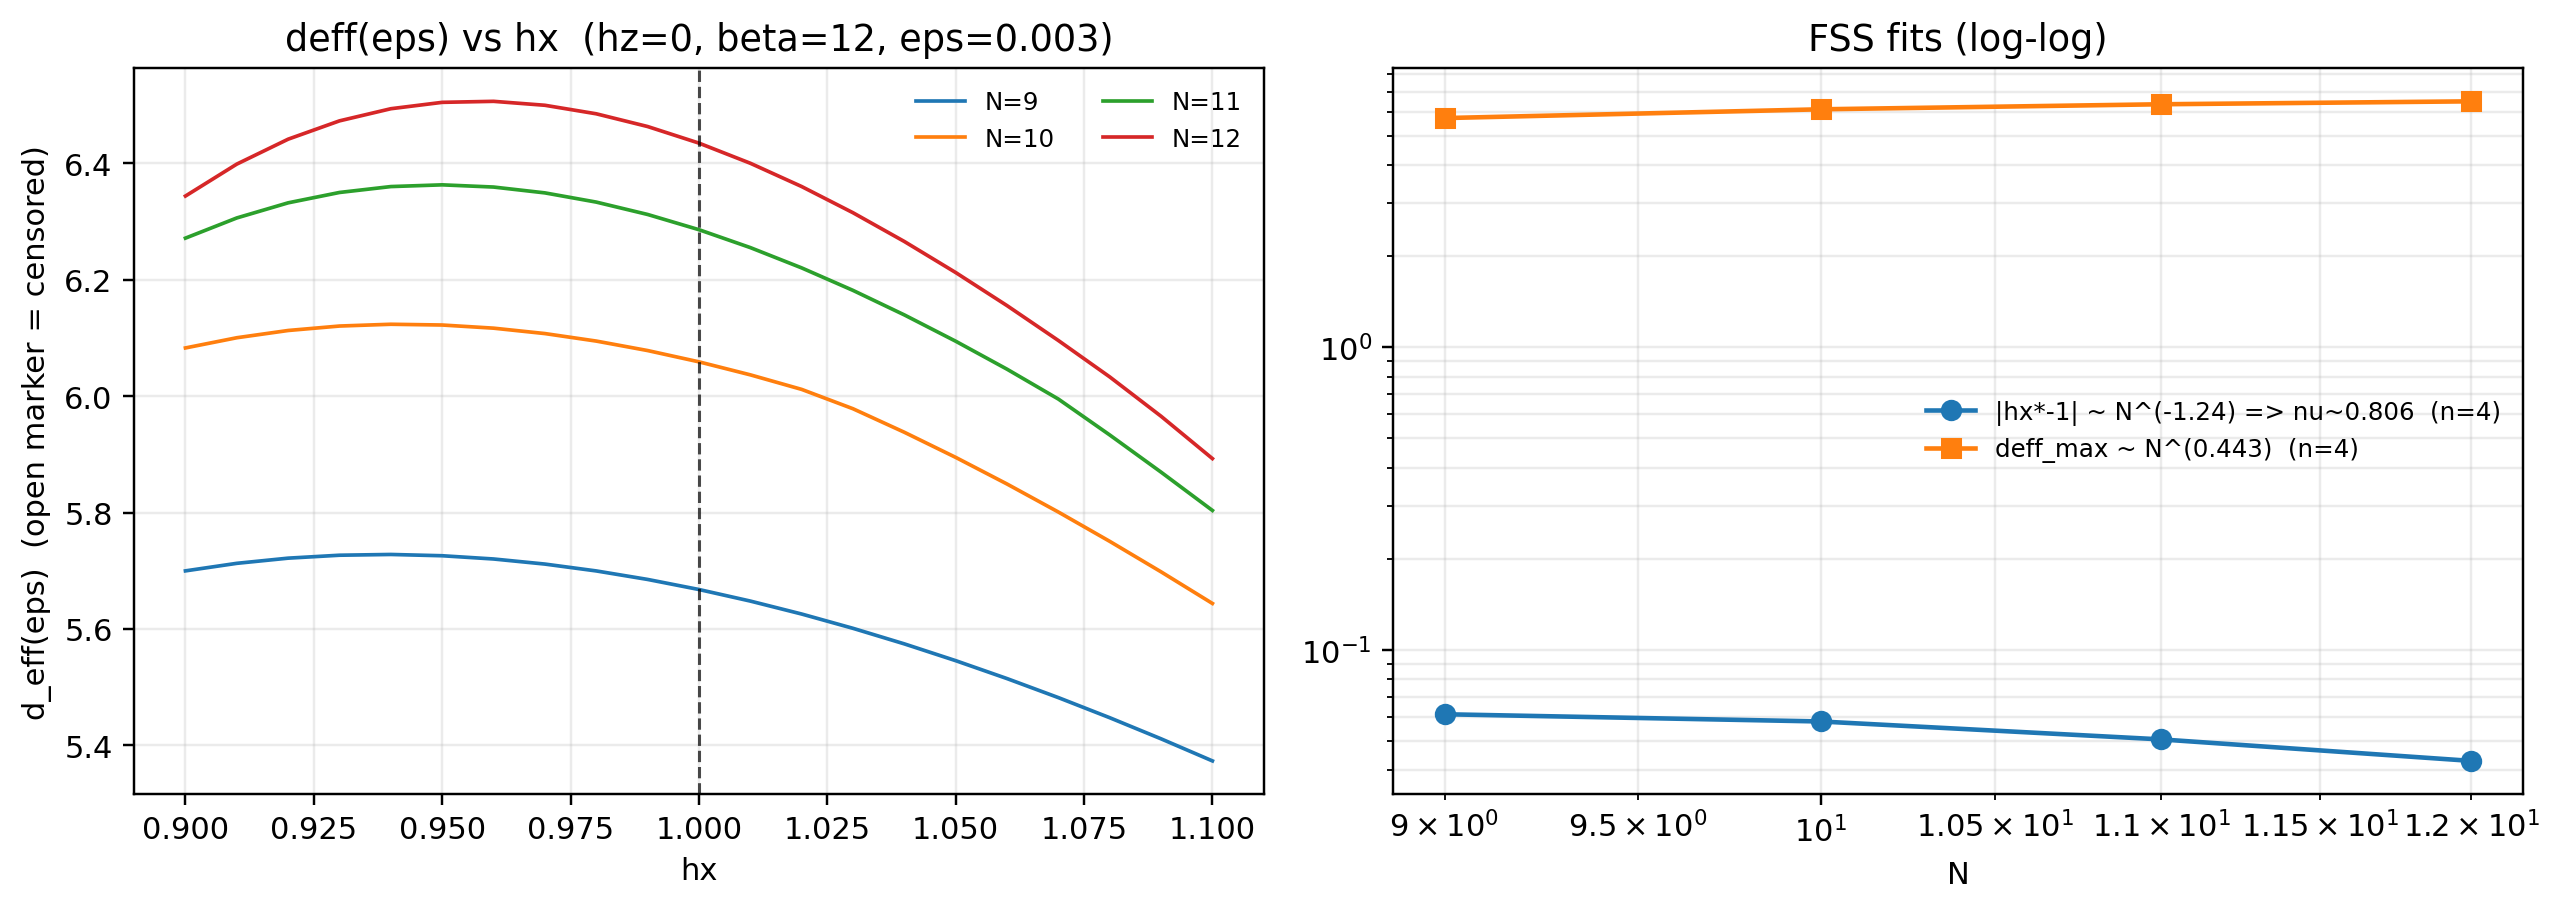
\includegraphics[width=0.95\textwidth]{fig1_eps3e3.png}
\caption{$\varepsilon = 3\times10^{-3}$, $\beta = 12$, $h_z = 0$ (v1
figure, unchanged). Left: $\deff$ vs $h_x$ for $N \in \{9,\dots,12\}$.
Right: log-log fits (read per Remarks~\ref{rem:baseline} and
\ref{rem:form}).}
\label{fig:e3}
\end{figure}
\begin{figure}[h]\centering
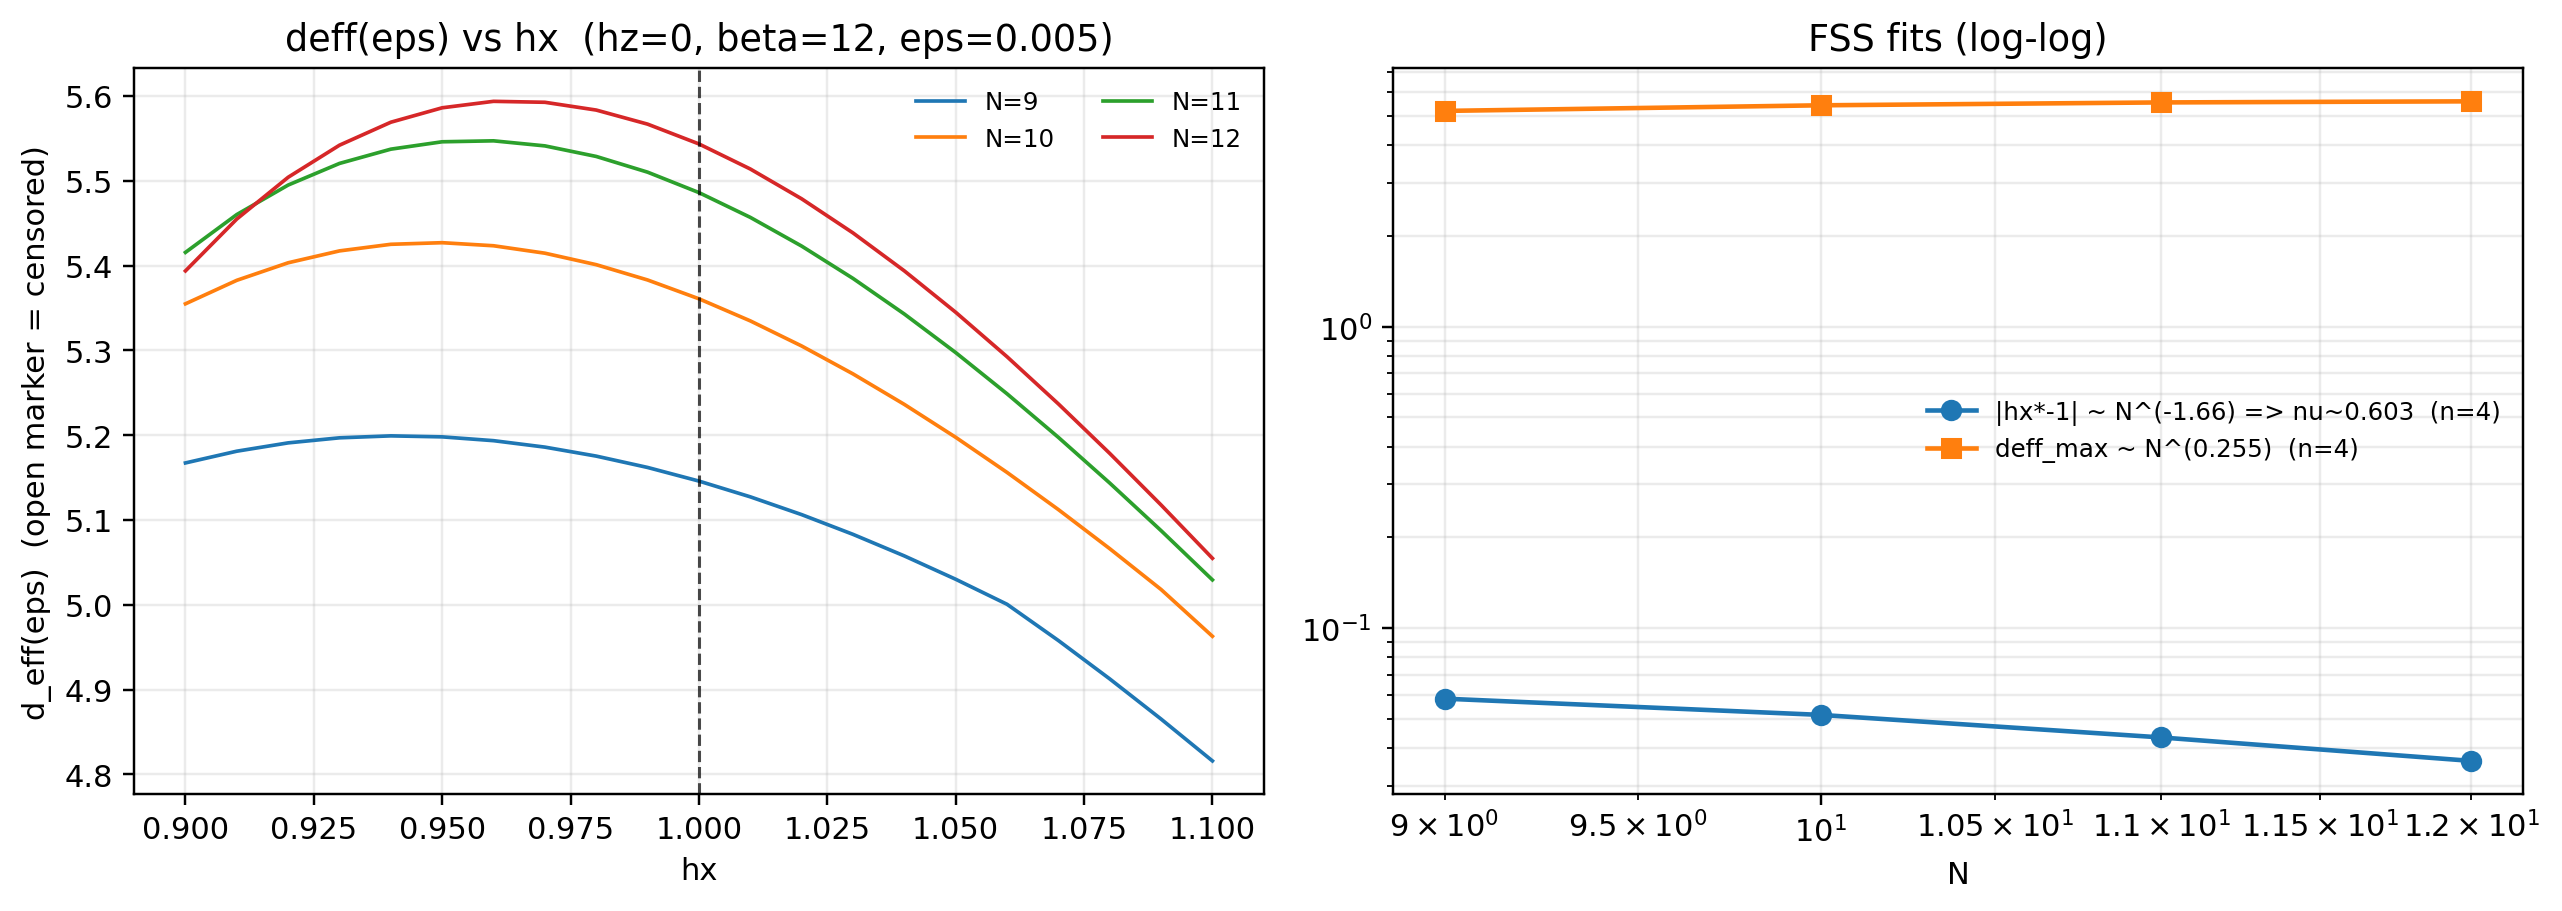
\includegraphics[width=0.95\textwidth]{fig2_eps5e3.png}
\caption{As above, $\varepsilon = 5\times10^{-3}$ (v1 figure, unchanged).}
\label{fig:e5}
\end{figure}

\section{Verification suite (added in v2)}
\texttt{verification/2601-0040/verify\_2601\_0040.py} (regenerable ED;
chunked JSON cache; default $N \in \{8, 9, 10\}$): reproduces v1's
Table~1 entries exactly where overlapping; computes the off-critical
baseline and critical enhancement of Remark~\ref{rem:baseline}; performs
the three-way functional-form comparison of Remark~\ref{rem:form};
verifies monotonicity of $E_{\rm best}$ and censoring-free status of the
chosen thresholds.

\section{Discussion}
The peak height grows monotonically with $N$ and the peak location
drifts toward the critical region -- both robust. What v2 sharpens is
the reading: the growth exponent is geometry-contaminated
(Remark~\ref{rem:baseline}) and form/window-dependent
(Remark~\ref{rem:form}); the baseline-subtracted critical enhancement is
the recommended object for future scaling studies, ideally under a
fixed-$|C|$ protocol with larger sizes (tensor networks), and compared
against CMI-based diagnostics as in 2601.0038 v2.

\section*{Note added in v2}
No v1 number is changed; Tables~1--2 and both figures stand, and the
suite reproduces Table~1 to all reported digits where sizes overlap. v2
adds the two caveats a referee would demand -- the $|C|$/baseline
confound (Remark~\ref{rem:baseline}, with the critical enhancement
$\Delta$ shown to survive) and functional-form/window dependence of
$\kappa$ (Remark~\ref{rem:form}) -- plus series positioning (v1 cited no
companion papers) and the regenerable verification suite.

\begin{thebibliography}{6}
\bibitem{Petz} D. Petz, Commun. Math. Phys. \textbf{105} (1986)
123--131.
\bibitem{Sachdev} S. Sachdev, \emph{Quantum Phase Transitions}, 2nd ed.,
Cambridge University Press (2011).
\bibitem{S0038} L. Eriksson, ai.viXra:2601.0038 (2026; v2 2026).
\bibitem{S0035} L. Eriksson, ai.viXra:2601.0035 (2026; v2 2026).
\bibitem{S0101} L. Eriksson, ai.viXra:2512.0101 (2025; v2 2026).
\end{thebibliography}
\end{document}
